% ============================================================================
%  INFORME COMPLETO — UN SOLO ARCHIVO
%  Desarrollo de un Sistema Móvil para la Visualización Interactiva de
%  Escenarios Deportivos a Nivel Nacional
%  Módulo de Inscripción a Eventos (Examen Integrador - PDF 7)
%
%  Compilar con: pdflatex → bibtex → pdflatex → pdflatex
%  O subir a Overleaf tal cual (Overleaf maneja la cadena automáticamente).
% ============================================================================

\documentclass[12pt,letterpaper]{article}

% ============================================================================
%  PREÁMBULO / FORMATO DEL INFORME  (normas APA · tipografía Helvetica/Arial)
% ============================================================================

% --- Idioma y codificación --------------------------------------------------
\RequirePackage[spanish,es-tabla]{babel}
\RequirePackage[T1]{fontenc}
\RequirePackage[utf8]{inputenc}

% --- Tipografía Arial (Helvetica a escala visual de 12 pt) ------------------
\RequirePackage[scaled=0.96]{helvet}
\renewcommand{\familydefault}{\sfdefault}

% --- Márgenes de 1 pulgada en papel carta (APA 7) ---------------------------
\RequirePackage[letterpaper,top=1in,bottom=1in,left=1in,right=1in]{geometry}

% --- Interlineado doble (APA 7) ---------------------------------------------
\RequirePackage[doublespacing]{setspace}

% --- Pie de página: línea horizontal y número de página a la derecha ---------
\RequirePackage{fancyhdr}
\setlength{\headheight}{17pt}
\setlength{\headsep}{25pt}
\pagestyle{fancy}
\fancyhf{}
\fancyfoot[R]{\thepage}
\renewcommand{\headrulewidth}{0pt}
\renewcommand{\footrulewidth}{0.4pt}
\fancypagestyle{plain}{%
  \fancyhf{}%
  \fancyfoot[R]{\thepage}%
  \renewcommand{\headrulewidth}{0pt}%
  \renewcommand{\footrulewidth}{0.4pt}%
}

% --- Jerarquía de títulos estilo APA ----------------------------------------
\RequirePackage{titlesec}
\titleformat{\section}{\bfseries\Large}{\thesection}{0.6em}{}
\titlespacing*{\section}{0pt}{12pt}{6pt}
\titleformat{\subsection}{\bfseries\large}{\thesubsection}{0.6em}{}
\titlespacing*{\subsection}{0pt}{12pt}{6pt}
\titleformat{\subsubsection}{\bfseries\normalsize\itshape}{\thesubsubsection}{0.6em}{}
\titlespacing*{\subsubsection}{0pt}{6pt}{6pt}

% --- Párrafos ---------------------------------------------------------------
\setlength{\parindent}{0pt}
\setlength{\parskip}{6pt}
\setlength{\emergencystretch}{3em}

% --- Tablas y figuras --------------------------------------------------------
\RequirePackage{booktabs}
\RequirePackage{array}
\RequirePackage{float}
\setlength{\tabcolsep}{3pt}
\renewcommand{\arraystretch}{1.3}
\RequirePackage{caption}
\AtBeginDocument{%
  \renewcommand{\figurename}{FIGURA}%
  \renewcommand{\tablename}{TABLA}%
}
\captionsetup{font=small, labelfont=bf, textfont=normal, singlelinecheck=true, skip=6pt}
\captionsetup[table]{labelsep=colon, position=above, justification=centering}
\captionsetup[figure]{labelsep=colon, position=above, justification=centering}

\newenvironment{tablaAPA}{\setstretch{1}\small}{}

% --- Fuente de figuras y tablas ----------------------------------------------
\newsavebox{\cajaContenido}
\newcommand{\contenidoConFuente}[2]{%
  \begin{lrbox}{\cajaContenido}#1\end{lrbox}%
  \parbox{\wd\cajaContenido}{%
    \usebox{\cajaContenido}\par
    \vspace{6pt}%
    {\setstretch{1}\footnotesize\textbf{FUENTE:} #2}%
  }%
}
\newcommand{\fuenteAPA}[1]{%
  \vspace{4pt}%
  {\setstretch{1}\footnotesize\textbf{FUENTE:} #1}%
}
\newcommand{\figuraAPA}[4]{%
  \begin{lrbox}{\cajaContenido}#3\end{lrbox}%
  \noindent
  \if\relax\detokenize{#1}\relax
    \captionsetup{width=\linewidth}\captionof{figure}{#2}%
  \else
    \captionsetup{width=\linewidth}\captionof{figure}{#2}\label{#1}%
  \fi
  \par
  \begin{center}%
    \parbox{\wd\cajaContenido}{%
      \setstretch{1}%
      \usebox{\cajaContenido}%
    }%
  \end{center}%
  \vspace{6pt}%
  {\setstretch{1}\footnotesize\textbf{FUENTE:} #4}%
}

% --- Gráficos y diagramas ----------------------------------------------------
\RequirePackage{graphicx}
\graphicspath{{figuras/}}
\newsavebox{\imagenBox}
\newcommand{\figuraSegura}[3][0.90]{%
  \begin{lrbox}{\imagenBox}
    \includegraphics[width=\textwidth,height=0.6\textheight,keepaspectratio]{#2}%
  \end{lrbox}
  \ifdim \wd\imagenBox > \textwidth
    \begin{center}
      \resizebox{\textwidth}{!}{\usebox{\imagenBox}}%
    \end{center}
  \else
    \begin{center}
      \usebox{\imagenBox}%
    \end{center}
  \fi
}
\RequirePackage{tikz}
\usetikzlibrary{shapes.geometric, arrows.meta, positioning, calc, fit}

% --- Código fuente -----------------------------------------------------------
\RequirePackage{listings}
\RequirePackage{xcolor}
\definecolor{codigofondo}{RGB}{245,245,245}
\lstset{
  basicstyle=\small\sffamily,
  backgroundcolor=\color{codigofondo},
  frame=single,
  breaklines=true,
  literate={ó}{{\'o}}1 {é}{{\'e}}1 {á}{{\'a}}1 {ú}{{\'u}}1 {ñ}{{\~n}}1
           {Ó}{{\'O}}1 {É}{{\'E}}1 {Á}{{\'A}}1 {Ú}{{\'U}}1 {Ñ}{{\~N}}1
           {í}{{\'i}}1 {Í}{{\'I}}1
           {¿}{{?}}1 {¡}{{!}}1
}

% --- Terminal ----------------------------------------------------------------
\definecolor{termbg}{RGB}{40,44,52}
\definecolor{termfg}{RGB}{220,220,220}
\definecolor{termcmd}{RGB}{97,175,239}
\definecolor{termout}{RGB}{171,178,191}
\definecolor{termok}{RGB}{152,195,121}
\lstdefinestyle{terminal}{
  basicstyle=\small\sffamily\color{termfg},
  backgroundcolor=\color{termbg},
  rulecolor=\color{termbg},
  frame=single,
  breaklines=true
}

% --- Listas, matemáticas y microtipografía -----------------------------------
\RequirePackage{enumitem}
\setlist{itemsep=2pt, parsep=0pt, topsep=6pt, partopsep=0pt}
\RequirePackage{amsmath}
\RequirePackage{amssymb}
\RequirePackage{microtype}

% --- Índices ----------------------------------------------------------------
\RequirePackage{tocloft}
\setcounter{tocdepth}{3}
\setcounter{secnumdepth}{3}
\setlength{\cftsecnumwidth}{2.8em}
\setlength{\cftsubsecnumwidth}{3.8em}
\setlength{\cftsubsubsecnumwidth}{4.6em}
\renewcommand{\cftpartfont}{\bfseries}
\renewcommand{\cftpartpagefont}{\bfseries}
\setlength{\cftbeforepartskip}{1.5em}
\renewcommand{\cfttoctitlefont}{\hfill\Large\bfseries}
\renewcommand{\cftaftertoctitle}{\hfill}
\renewcommand{\cftlottitlefont}{\hfill\Large\bfseries}
\renewcommand{\cftafterlottitle}{\hfill}
\renewcommand{\cftloftitlefont}{\hfill\Large\bfseries}
\renewcommand{\cftafterloftitle}{\hfill}
\renewcommand{\cftfigpresnum}{\textbf{FIGURA }}
\renewcommand{\cfttabpresnum}{\textbf{TABLA }}
\renewcommand{\cftfigaftersnum}{:}
\renewcommand{\cfttabaftersnum}{:}
\setlength{\cftfignumwidth}{7em}
\setlength{\cfttabnumwidth}{7em}

% --- Hipervínculos -----------------------------------------------------------
\RequirePackage[colorlinks=true, linkcolor=black, urlcolor=blue, citecolor=black]{hyperref}

% --- Referencias en formato APA (paquete apacite) ----------------------------
\RequirePackage[natbibapa]{apacite}

% --- Encabezado de capítulo ---------------------------------------------------
\newcommand{\textoEncabezado}[2]{%
  \parbox{\headwidth}{\raggedleft
    \setstretch{1}%
    \textbf{#1}%
    \\[-6pt]{\rule{\headwidth}{0.4pt}}%
    \if\relax\detokenize{#2}\relax\else\\[2pt]\textbf{#2}\fi
  }%
}
\newcommand{\encabezadoCapitulo}[2]{%
  \fancyhead[C]{\textoEncabezado{#1}{#2}}%
}

% --- Carátula de capítulo (1 hoja completa) -----------------------------------
\newcounter{capitulo}
\renewcommand{\thesection}{\arabic{capitulo}.\arabic{section}}
\renewcommand{\theHsection}{\arabic{capitulo}.\arabic{section}}
\renewcommand{\theHsubsection}{\theHsection.\arabic{subsection}}
\renewcommand{\theHsubsubsection}{\theHsubsection.\arabic{subsubsection}}
\newcommand{\caratulaCapitulo}[2]{%
  \clearpage
  \refstepcounter{capitulo}%
  \setcounter{section}{0}%
  \pdfbookmark[0]{#1:\ #2}{capitulo.\arabic{capitulo}}%
  \addtocontents{toc}{%
    \protect\contentsline{part}{#1\protect\\#2}{\thepage}{\@currentHref}%
  }%
  \encabezadoCapitulo{#2}{}%
  \fancypagestyle{primeraCap}{%
    \fancyhf{}%
    \fancyfoot[R]{\thepage}%
    \fancyhead[C]{\textoEncabezado{#2}{#1}}%
    \renewcommand{\headrulewidth}{0pt}%
    \renewcommand{\footrulewidth}{0.4pt}%
  }%
  \thispagestyle{empty}%
  \begin{center}
    \vspace*{6.2cm}
    {\bfseries\Huge #1 \par}
    \vspace{1.7cm}
    {\bfseries\LARGE #2 \par}
  \end{center}
  \clearpage
  \addtocounter{page}{-1}%
  \thispagestyle{primeraCap}%
}

% ============================================================================
%  DATOS DEL DOCUMENTO
% ============================================================================
\newcommand{\tituloDocumento}{Desarrollo de un Sistema M\'ovil para la
  Visualizaci\'on Interactiva de Escenarios Deportivos a Nivel Nacional}
\newcommand{\nombreApp}{DeporteYa}
\newcommand{\equipo}{Sudoers}
\newcommand{\integrantes}{%
  Joaquin Alessandro Felipez Rojas \par}
\newcommand{\universidad}{Universidad Privada Domingo Savio}
\newcommand{\facultad}{Facultad de Ingenier\'ia}
\newcommand{\carrera}{Ingenier\'ia en Sistemas}
\newcommand{\asignatura}{Aplicaciones M\'oviles I}
\newcommand{\docente}{Vladimir Wilmar Rojas Condori}
\newcommand{\ciudad}{Cochabamba--Bolivia}
\newcommand{\fechaEntrega}{\today}

\begin{document}

% --- Numeración: romano antes del Capítulo I, arábigo desde el Capítulo I ---
\pagenumbering{roman}

% ============================================================================
%  PORTADA
% ============================================================================
\begin{titlepage}
  \thispagestyle{empty}
  \setstretch{1}
  \setlength{\parskip}{0pt}

  \begin{center}
    \vspace*{0.6cm}

    {\bfseries\fontsize{20}{24}\selectfont \universidad \par}
    {\bfseries\fontsize{18}{22}\selectfont \facultad \par}
    {\bfseries\fontsize{16}{19}\selectfont \carrera \par}

    \vspace{0.8cm}

    
\includegraphics[width=0.30\textwidth]{figuras/logo-upds.png}\par

    \vspace{0.9cm}

    {\bfseries\Large \tituloDocumento \par}

    \vspace{1.0cm}

    {\large \integrantes \par}

    \vspace{1.0cm}

    {\normalsize \textbf{Asignatura:} \asignatura \par}
    {\normalsize \textbf{Docente:} \docente \par}
    {\normalsize \textbf{Fecha de entrega:} \fechaEntrega \par}

    \vspace{1.1cm}

    {\normalsize \textbf{Equipo:} \equipo \par}

    \vspace{0.9cm}

    {\normalsize \ciudad \par}

    \vspace{0.2cm}

    {\normalsize 2026 \par}
  \end{center}
\end{titlepage}

% ============================================================================
%  RESUMEN
% ============================================================================
\begin{abstract}
\noindent
\textbf{Objetivo:} Desarrollar e integrar un m\'odulo de inscripci\'on a
eventos deportivos en la aplicaci\'on m\'ovil \nombreApp{}, que permita a los
usuarios registrarse, cancelar inscripciones y consultar su estado de
inscripci\'on desde la interfaz de la aplicaci\'on.

\medskip
\noindent
\textbf{Metodolog\'ia:} Se sigui\'o un proceso de an\'alisis de necesidades,
dise\~no de interfaz, implementaci\'on de backend (Supabase/PostgreSQL),
desarrollo de componentes React Native con Expo, y pruebas de integraci\'on.
El m\'odulo se bas\'o en la arquitectura existente del proyecto, reutilizando
hooks de React Query, el sistema de dise\~no de colores y los patrones de
navegaci\'on con Expo Router.

\medskip
\noindent
\textbf{Resultados:} Se implement\'o una tabla \texttt{event\_registrations}
con pol\'iticas RLS granulares, hooks personalizados para las operaciones
CRUD, un componente de bot\'on de inscci\'on con estados visuales, y una
secci\'on de ``Mis inscripciones'' en el perfil del usuario. El m\'odulo
cumple con los requisitos de validaci\'on, manejo de errores, persistencia
en la nube e integraci\'on con la aplicaci\'on existente.

\medskip
\noindent
\textbf{Palabras clave:} inscripci\'on a eventos, React Native, Expo,
Supabase, PostgreSQL, CRUD, RLS, aplicaciones m\'oviles.
\end{abstract}

% --- Índices ---
\newpage
\tableofcontents
\newpage
\listoftables
\newpage
\listoffigures
\clearpage

% --- Cambio a numeración arábiga ---
\clearpage
\pagenumbering{arabic}

% ============================================================================
%  CAPÍTULO III: DESARROLLO DEL MÓDULO DE INSCRIPCIÓN A EVENTOS
% ============================================================================

\caratulaCapitulo{CAP\'ITULO III}{DESARROLLO DEL M\'ODULO DE INSCRIPCI\'ON A EVENTOS}

% ---------------------------------------------------------------------------
%  3.1 ANÁLISIS DE LA NECESIDAD
% ---------------------------------------------------------------------------
\section{An\'alisis de la necesidad}

\subsection{Contexto del proyecto}

La aplicaci\'on \nombreApp{} es un sistema m\'ovil para la
visualizaci\'on interactiva de escenarios deportivos a nivel nacional
en Bolivia. Permite a los ciudadanos localizar y acceder a informaci\'on
confiable sobre infraestructura deportiva del pa\'is, incluyendo
estadios, coliseos, canchas m\'ultiples y polideportivos.

El sistema actual cuenta con las siguientes funcionalidades principales:

\begin{itemize}
  \item \textbf{Mapa interactivo:} Ubicaci\'on de escenarios en un mapa
    con MapLibre (nativo y web).
  \item \textbf{Detalle de escenario:} Informaci\'on completa incluyendo
    imagenes, deportes disponibles, horarios y eventos pr\'oximos.
  \item \textbf{Favoritos:} Guardado de escenarios de inter\'es del
    usuario.
  \item \textbf{B\'usqueda:} B\'usqueda por nombre, deporte o
    ubicaci\'on.
  \item \textbf{Gesti\'on:} CRUD de escenarios para roles admin y gestor.
  \item \textbf{Visor 360:} Exploraci\'on panor\'amica de sectores del
    estadio.
  \item \textbf{Eventos:} Creaci\'on y consulta de eventos deportivos
    asociados a escenarios.
\end{itemize}

\subsection{El problema identificado}

Si bien la aplicaci\'on permite \textit{ver} los eventos pr\'oximos
asociados a cada escenario, no existe un mecanismo para que los
usuarios \textbf{se inscriban} a dichos eventos. Esto genera las
siguientes limitaciones:

\begin{enumerate}
  \item \textbf{Sin seguimiento:} El usuario no tiene forma de indicar
    qu\'e eventos le interesan asistir.
  \item \textbf{Sin conteo de asistencia:} No se conoce cu\'antas
    personas planean asistir a cada evento.
  \item \textbf{Sin recordatorios:} No hay base para futuras
    notificaciones de eventos pr\'oximos.
  \item \textbf{Experiencia incompleta:} La app muestra eventos pero
    no permite interactuar con ellos de manera significativa.
\end{enumerate}

\subsection{Justificaci\'on del nuevo m\'odulo}

La incorporaci\'on de un m\'odulo de inscripci\'on a eventos resuelve
estas limitaciones y aporta valor tanto al usuario final como al
gestor del escenario:

\begin{itemize}
  \item \textbf{Para el usuario:} Puede inscribirse a eventos de
    inter\'es, cancelar su inscripci\'on, y consultar sus inscripciones
    desde su perfil.
  \item \textbf{Para el gestor:} Puede ver cu\'antas personas est\'an
    inscritas en cada evento, lo que le permite planificar
    log\'istica y capacidad.
  \item \textbf{Para el admin:} Tiene visibilidad completa de todas las
    inscripciones del sistema.
\end{itemize}

% ---------------------------------------------------------------------------
%  3.2 DEFINICIÓN DE LA FUNCIONALIDAD
% ---------------------------------------------------------------------------
\section{Definici\'on de la funcionalidad}

\subsection{Nombre de la funcionalidad}

Inscripci\'on a Eventos Deportivos.

\subsection{Objetivo}

Permitir a los usuarios autenticados inscribirse a eventos deportivos
asociados a los escenarios, cancelar dichas inscripciones, y consultar
su estado desde la interfaz de la aplicaci\'on.

\subsection{Usuarios involucrados}

\begin{table}[H]
\centering
\begin{tabular}{@{}lll@{}}
\toprule
\textbf{Rol} & \textbf{Acciones} & \textbf{Restricciones} \\
\midrule
Asistente & Inscribirse, cancelar, ver sus inscripciones & Solo sus propias \\
Gestor & Ver inscripciones de sus eventos & Solo sus escenarios \\
Admin & Ver todas las inscripciones, eliminar cualquiera & Sin restricciones \\
\bottomrule
\end{tabular}
\caption{Roles y permisos del m\'odulo}
\end{table}

\subsection{Flujo de funcionamiento}

El flujo principal de la funcionalidad se describe a continuaci\'on:

\begin{figure}[H]
\centering
\begin{tikzpicture}[
  node distance=0.8cm,
  caja/.style={rectangle, draw=black!60, rounded corners,
    minimum width=2.8cm, minimum height=0.7cm, align=center,
    font=\footnotesize, fill=blue!5},
  flecha/.style={-Stealth, thick}
]
  \node[caja] (inicio) {Usuario};
  \node[caja, right=of inicio] (escenario) {Detalle del\\escenario};
  \node[caja, right=of escenario] (evento) {Selecciona\\evento};
  \node[caja, below=of evento] (validar) {Validar\\datos};
  \node[caja, left=of validar] (guardar) {Guardar en\\Supabase};
  \node[caja, left=of guardar] (exito) {Inscripci\'on\\confirmada};
  \node[caja, below=of validar] (error) {Mostrar\\error};

  \draw[flecha] (inicio) -- (escenario);
  \draw[flecha] (escenario) -- (evento);
  \draw[flecha] (evento) -- (validar);
  \draw[flecha] (validar) -- node[above, font=\scriptsize] {V\'alido} (guardar);
  \draw[flecha] (validar) -- node[right, font=\scriptsize] {Inv\'alido} (error);
  \draw[flecha] (guardar) -- (exito);
\end{tikzpicture}
\caption{Flujo de inscripci\'on a eventos}
\end{figure}

\subsection{Operaciones CRUD}

El m\'odulo implementa las siguientes operaciones sobre la tabla
\texttt{event\_registrations}:

\begin{table}[H]
\centering
\begin{tabular}{@{}llp{6cm}@{}}
\toprule
\textbf{Operaci\'on} & \textbf{M\'etodo HTTP} & \textbf{Descripci\'on} \\
\midrule
CREATE & INSERT & El usuario se inscribe a un evento \\
READ & SELECT & Consultar inscripciones propias o de un evento \\
UPDATE & UPDATE & Cambiar estado de inscripci\'on (no implementado
  actualmente, se usa DELETE) \\
DELETE & DELETE & Cancelar inscripci\'on \\
\bottomrule
\end{tabular}
\caption{Operaciones CRUD del m\'odulo}
\end{table}

\subsection{Persistencia}

Toda la informaci\'on de inscripciones se almacena en Supabase
(PostgreSQL), ya que requiere persistencia centralizada:
\begin{itemize}
  \item \textbf{Inspecci\'on:} Disponible para todos los dispositivos
    del usuario (multi-dispositivo).
  \item \textbf{Gesti\'on:} Los gestores y admins pueden consultar
    inscripciones desde cualquier punto.
  \item \textbf{Seguridad:} Las pol\'iticas RLS garantizan que cada
    usuario solo vea sus propias inscripciones (salvo admin/gestor).
\end{itemize}

% ---------------------------------------------------------------------------
%  3.3 DISEÑO DE LA INTERFAZ
% ---------------------------------------------------------------------------
\section{Dise\~no de la interfaz}

\subsection{Principios de dise\~no}

La interfaz del m\'odulo de inscripci\'on sigue los principios de
dise\~no establecidos en el proyecto:

\begin{itemize}
  \item \textbf{Consistencia visual:} Se reutiliz\'o el sistema de
    colores existente (\texttt{colors.ts}), el espaciado
    (\texttt{spacing.ts}) y la tipograf\'ia (\texttt{fontSize},
    \texttt{fontWeight}).
  \item \textbf{Coherencia con la app:} Los botones de inscripci\'on
    siguen el mismo estilo que el bot\'on de favoritos.
  \item \textbf{Retroalimentaci\'on visual:} El bot\'on cambia de
    apariencia al inscribirse/cancelar.
  \item \textbf{Accesibilidad:} Iconos descriptivos (Ionicons) y
    contraste adecuado.
\end{itemize}

\subsection{Pantallas del m\'odulo}

El m\'odulo se integra en dos pantallas existentes:

\subsubsection*{1. Detalle del escenario (secci\'on de eventos)}

Cada tarjeta de evento en la pantalla de detalle ahora incluye:

\begin{itemize}
  \item Nombre, fecha y hora del evento
  \item Descripci\'on (si existe)
  \item Conteo de inscritos (ej: ``3 inscritos'')
  \item Bot\'on de inscripci\'on/desinscripci\'on
\end{itemize}

\begin{figure}[H]
\centering
\figuraAPA{fig:diseno-evento-detalle}{Dise\~no de la tarjeta de evento con bot\'on de inscripci\'on}{%
  \begin{tikzpicture}[
    box/.style={rectangle, draw=black!60, rounded corners,
      minimum width=5cm, minimum height=3.5cm, align=left,
      font=\footnotesize, fill=gray!5, inner sep=8pt}
  ]
    \node[box] {
      \textbf{Nombre del Evento} \\
      \textit{Fecha: 2026-09-15 · Hora: 20:00} \\
      \\
      Descripci\'on del evento deportivo \\
      \\
      \textcolor{green!60!black}{\checkmark} 5 inscritos \\
      \\
      \textcolor{blue}{\textbf{[Inscribirse]}} \quad
      \textcolor{red}{\textbf{[Eliminar]}}
    };
  \end{tikzpicture}
}{Elaboraci\'on propia (dise\~no del componente).}
\end{figure}

\subsubsection*{2. Perfil del usuario (secci\'on ``Mis inscripciones'')}

En la pantalla de perfil se agreg\'o una nueva secci\'on que muestra
todas las inscripciones activas del usuario:

\begin{itemize}
  \item Icono de confirmaci\'on (checkmark verde)
  \item Fecha de inscripci\'on
  \item Estado vac\'io cuando no hay inscripciones
\end{itemize}

\begin{figure}[H]
\centering
\figuraAPA{fig:diseno-perfil-inscripciones}{Secci\'on ``Mis inscripciones'' en el perfil}{%
  \begin{tikzpicture}[
    box/.style={rectangle, draw=black!60, rounded corners,
      minimum width=5cm, minimum height=3cm, align=left,
      font=\footnotesize, fill=gray!5, inner sep=8pt}
  ]
    \node[box] {
      \textbf{MIS INSCRIPCIONES A EVENTOS} \\
      \\
      \textcolor{green!60!black}{$\bigcirc$} Evento \\
      \quad Inscrito el 15 de septiembre \\
      \\
      \textcolor{green!60!black}{$\bigcirc$} Evento \\
      \quad Inscrito el 20 de octubre
    };
  \end{tikzpicture}
}{Elaboraci\'on propia (dise\~no del componente).}
\end{figure}

\subsection{Estados visuales del bot\'on}

El bot\'on de inscripci\'on tiene tres estados:

\begin{table}[H]
\centering
\begin{tabular}{@{}lll@{}}
\toprule
\textbf{Estado} & \textbf{Apariencia} & \textbf{Comportamiento} \\
\midrule
No inscrito & Borde azul, fondo blanco & Al tocar, inscribe \\
Inscrito & Fondo azul, texto blanco & Al tocar, pide confirmaci\'on \\
Cargando & Indicador de progreso & Deshabilitado \\
\bottomrule
\end{tabular}
\caption{Estados del bot\'on de inscripci\'on}
\end{table}

% ---------------------------------------------------------------------------
%  3.4 MODELO DE DATOS
% ---------------------------------------------------------------------------
\section{Modelo de datos}

\subsection{Tabla \texttt{event\_registrations}}

Se cre\'o una nueva tabla en PostgreSQL mediante la migraci\'on
\texttt{011\_event\_registrations.sql}:

\begin{verbatim}
CREATE TABLE public.event_registrations (
  id UUID PRIMARY KEY DEFAULT gen_random_uuid(),
  user_id UUID NOT NULL REFERENCES public.profiles(id)
    ON DELETE CASCADE,
  event_id UUID NOT NULL REFERENCES public.events(id)
    ON DELETE CASCADE,
  status TEXT NOT NULL DEFAULT 'confirmed'
    CHECK (status IN ('confirmed', 'cancelled', 'waitlist')),
  registered_at TIMESTAMPTZ NOT NULL DEFAULT NOW(),
  UNIQUE (user_id, event_id)
);
\end{verbatim}

\subsection{Campos de la tabla}

\begin{table}[H]
\centering
\begin{tabular}{@{}lllp{5cm}@{}}
\toprule
\textbf{Campo} & \textbf{Tipo} & \textbf{Restricci\'on} &
  \textbf{Descripci\'on} \\
\midrule
id & UUID & PK, auto & Identificador \'unico \\
user\_id & UUID & FK $\to$ profiles & Usuario inscrito \\
event\_id & UUID & FK $\to$ events & Evento al que se inscribe \\
status & TEXT & CHECK, default & Estado: confirmed, cancelled,
  waitlist \\
registered\_at & TIMESTAMPTZ & default NOW() & Fecha de inscripci\'on \\
\bottomrule
\end{tabular}
\caption{Campos de la tabla \texttt{event\_registrations}}
\end{table}

\subsection{Relaciones}

\begin{figure}[H]
\centering
\begin{tikzpicture}[
  node distance=1.5cm,
  entity/.style={rectangle, draw=black, thick, minimum width=2.2cm,
    minimum height=0.8cm, align=center, font=\footnotesize,
    fill=blue!8},
  relation/.style={-Stealth, thick}
]
  \node[entity] (profiles) {profiles};
  \node[entity, right=of profiles] (reg) {event\_\\registrations};
  \node[entity, right=of reg] (events) {events};

  \draw[relation] (profiles) -- node[above, font=\scriptsize]
    {user\_id} (reg);
  \draw[relation] (reg) -- node[above, font=\scriptsize]
    {event\_id} (events);
\end{tikzpicture}
\caption{Diagrama de relaciones del m\'odulo}
\end{figure}

\subsection{Pol\'iticas RLS (Row Level Security)}

La tabla habilita RLS con las siguientes pol\'iticas:

\begin{table}[H]
\centering
\small
\begin{tabular}{@{}lp{4.5cm}p{4.5cm}@{}}
\toprule
\textbf{Pol\'itica} & \textbf{Acci\'on} & \textbf{Condici\'on} \\
\midrule
select\_own & SELECT & user\_id = auth.uid() \\
select\_admin & SELECT & Rol = admin \\
select\_gestor & SELECT & Es gestor del escenario \\
insert\_own & INSERT & user\_id = auth.uid() \\
update\_own & UPDATE & user\_id = auth.uid() \\
delete\_own\_or\_admin & DELETE & user\_id = auth.uid() o admin \\
\bottomrule
\end{tabular}
\caption{Pol\'iticas RLS de la tabla \texttt{event\_registrations}}
\end{table}

\subsection{Vista \texttt{event\_registration\_counts}}

Se cre\'o una vista para obtener el conteo de inscripciones por evento:

\begin{verbatim}
CREATE OR REPLACE VIEW
  public.event_registration_counts AS
SELECT
  event_id,
  COUNT(*) FILTER (WHERE status = 'confirmed')
    AS confirmed_count,
  COUNT(*) FILTER (WHERE status = 'waitlist')
    AS waitlist_count
FROM public.event_registrations
GROUP BY event_id;
\end{verbatim}

% ---------------------------------------------------------------------------
%  3.5 IMPLEMENTACIÓN DEL BACKEND (Hooks de React Query)
% ---------------------------------------------------------------------------
\section{Implementaci\'on del backend}

\subsection{Hooks personalizados}

Se cre\'o el archivo \texttt{src/hooks/useEventRegistration.ts} con
cinco hooks que encapsulan toda la l\'ogica de comunicaci\'on con
Supabase:

\begin{enumerate}
  \item \textbf{useIsRegistered(userId, eventId):} Verifica si el
    usuario est\'a inscrito en un evento espec\'ifico.
  \item \textbf{useRegisterForEvent():} Inscribir al usuario en un
    evento.
  \item \textbf{useCancelRegistration():} Cancelar la inscripci\'on
    del usuario.
  \item \textbf{useMyRegistrations(userId):} Obtener todas las
    inscripciones activas del usuario.
  \item \textbf{useRegistrationCounts(eventIds):} Obtener el conteo
    de inscripciones para una lista de eventos.
\end{enumerate}

\subsection{Funciones de API}

Cada hook internamente llama a una funci\'on de API que interact\'ua
directamente con Supabase:

\subsubsection*{Verificar inscripci\'on}

\begin{verbatim}
async function checkRegistration(
  userId: string, eventId: string
): Promise<EventRegistration | null> {
  const { data, error } = await supabase
    .from('event_registrations')
    .select('*')
    .eq('user_id', userId)
    .eq('event_id', eventId)
    .in('status', ['confirmed', 'waitlist'])
    .maybeSingle();

  if (error) throw new Error(error.message);
  return data as EventRegistration | null;
}
\end{verbatim}

\subsubsection*{Inscribir en evento}

\begin{verbatim}
async function registerForEvent(
  userId: string, eventId: string
): Promise<EventRegistration> {
  const existing = await checkRegistration(userId, eventId);
  if (existing) {
    throw new Error('Ya estas inscrito en este evento');
  }

  const { data, error } = await supabase
    .from('event_registrations')
    .insert({
      user_id: userId,
      event_id: eventId,
      status: 'confirmed',
    })
    .select()
    .single();

  if (error) throw new Error(error.message);
  return data as EventRegistration;
}
\end{verbatim}

\subsubsection*{Cancelar inscripci\'on}

\begin{verbatim}
async function cancelRegistration(
  userId: string, eventId: string
): Promise<void> {
  const { error } = await supabase
    .from('event_registrations')
    .delete()
    .eq('user_id', userId)
    .eq('event_id', eventId);

  if (error) throw new Error(error.message);
}
\end{verbatim}

\subsection{Invalidaci\'on de cach\'e}

Todos los hooks utilizan \texttt{useQueryClient} para invalidar la
cach\'e despu\'es de cada operaci\'on, garantizando que la interfaz
se actualice con los datos m\'as recientes:

\begin{verbatim}
onSuccess: (_, variables) => {
  queryClient.invalidateQueries({
    queryKey: ['event-registration',
      variables.userId, variables.eventId],
  });
  queryClient.invalidateQueries({
    queryKey: ['event-registration-counts'],
  });
  queryClient.invalidateQueries({
    queryKey: ['my-event-registrations',
      variables.userId],
  });
},
\end{verbatim}

% ---------------------------------------------------------------------------
%  3.6 IMPLEMENTACIÓN DEL FRONTEND
% ---------------------------------------------------------------------------
\section{Implementaci\'on del frontend}

\subsection{Componente \texttt{EventRegistrationButton}}

Se cre\'o un componente reutilizable que gestiona el estado del bot\'on
de inscripci\'on:

\begin{verbatim}
function EventRegistrationButton({
  eventId, eventName, userId,
  isRegistering, isCancelling,
  onRegister, onCancel,
}: EventRegistrationButtonProps) {
  const { data: registration, isLoading } =
    useIsRegistered(userId, eventId);
  const isRegistered = !!registration;

  return (
    <TouchableOpacity
      style={[
        styles.registerButton,
        isRegistered && styles.registerButtonActive,
      ]}
      onPress={() => {
        if (isRegistered) {
          onCancel(eventId, eventName);
        } else {
          onRegister(eventId);
        }
      }}
      disabled={isLoadingState}
    >
      <Ionicons
        name={isRegistered
          ? 'checkmark-circle'
          : 'add-circle-outline'}
        size={16}
        color={isRegistered ? colors.white : colors.primary}
      />
      <Text style={...}>
        {isRegistered ? 'Inscrito' : 'Inscribirse'}
      </Text>
    </TouchableOpacity>
  );
}
\end{verbatim}

\subsection{Integraci\'on en el detalle del escenario}

En \texttt{src/app/scenario/[id].tsx} se modificaron las tarjetas de
evento para incluir el bot\'on de inscripci\'on y el conteo de
inscritos:

\begin{verbatim}
{scenario.events.map((event) => {
  const counts = registrationCounts?.[event.id];
  return (
    <View key={event.id} style={styles.eventCard}>
      {/* ... info del evento ... */}
      {counts && (
        <Text style={styles.registrationCount}>
          {counts.confirmed_count} inscrito(s)
        </Text>
      )}
      <View style={styles.eventActions}>
        {user && (
          <EventRegistrationButton
            eventId={event.id}
            userId={user.id}
            onRegister={handleRegister}
            onCancel={handleCancelRegistration}
          />
        )}
      </View>
    </View>
  );
})}
\end{verbatim}

\subsection{Secci\'on ``Mis inscripciones'' en el perfil}

En \texttt{src/app/(tabs)/profile.tsx} se agreg\'o el componente
\texttt{MyRegistrationsSection} que consulta y muestra las
inscripciones del usuario:

\begin{verbatim}
function MyRegistrationsSection({ userId }) {
  const { data: registrations, isLoading } =
    useMyRegistrations(userId);

  if (isLoading) return <ActivityIndicator />;
  if (registrations?.length > 0) {
    return (
      <View style={styles.infoCard}>
        {registrations.map((reg) => (
          <View key={reg.id}>
            <Ionicons name="checkmark-circle"
              color={colors.success} />
            <Text>Inscrito el {reg.registered_at}</Text>
          </View>
        ))}
      </View>
    );
  }
  return (
    <View style={styles.emptyRegistrations}>
      <Text>No tienes inscripciones aun</Text>
    </View>
  );
}
\end{verbatim}

\subsection{Estilos personalizados}

Se agregaron los siguientes estilos al archivo de estilos del
detalle del escenario:

\begin{table}[H]
\centering
\begin{tabular}{@{}ll@{}}
\toprule
\textbf{Estilo} & \textbf{Descripci\'on} \\
\midrule
eventActions & Contenedor flex para botones de acci\'on \\
registrationCount & Texto verde para conteo de inscritos \\
registerButton & Bot\'on con borde azul, fondo blanco \\
registerButtonActive & Bot\'on con fondo azul (inscrito) \\
registerButtonDisabled & Opacidad reducida (cargando) \\
registerButtonText & Texto azul del bot\'on \\
registerButtonTextActive & Texto blanco del bot\'on activo \\
\bottomrule
\end{tabular}
\caption{Estilos del m\'odulo de inscripci\'on}
\end{table}

% ---------------------------------------------------------------------------
%  3.7 VALIDACIONES Y MANEJO DE ERRORES
% ---------------------------------------------------------------------------
\section{Validaciones y manejo de errores}

\subsection{Validaciones implementadas}

El m\'odulo incluye las siguientes validaciones:

\begin{enumerate}
  \item \textbf{Autenticaci\'on:} Antes de inscribirse, se verifica
    que el usuario est\'a logueado. Si no lo est\'a, se muestra un
    alerta ``Iniciar sesi\'on''.

  \item \textbf{Duplicados:} La funci\'on \texttt{registerForEvent}
    verifica si ya existe una inscripci\'on activa antes de insertar.
    Si existe, lanza el error ``Ya est\'as inscrito en este evento''.

  \item \textbf{Restricci\'on SQL:} La tabla tiene una restricci\'on
    \texttt{UNIQUE (user\_id, event\_id)} que previene duplicados
    a nivel de base de datos.

  \item \textbf{Estado:} Solo se permiten los valores ``confirmed'',
    ``cancelled'' y ``waitlist'' mediante la restricci\'on CHECK.

  \item \textbf{Integridad referencial:} Las foreign keys
    \texttt{user\_id $\to$ profiles} y \texttt{event\_id $\to$ events}
    garantizan que las referencias sean v\'alidas.
\end{enumerate}

\subsection{Manejo de errores}

\subsubsection*{Errores de red / Supabase}

Todas las funciones de API capturan errores de Supabase y los
re-lanzan como \texttt{Error} con el mensaje descriptivo:

\begin{verbatim}
if (error) throw new Error(error.message);
\end{verbatim}

\subsubsection*{Errores en la interfaz}

Los handlers en React capturan los errores y muestran alertas:

\begin{verbatim}
const handleRegister = async (eventId) => {
  if (!user?.id) {
    Alert.alert('Iniciar sesion',
      'Debes iniciar sesion para inscribirte.');
    return;
  }
  try {
    await registerEvent({ userId: user.id, eventId });
  } catch (err) {
    const msg = err instanceof Error
      ? err.message
      : 'Error al inscribirte';
    Alert.alert('Error', msg);
  }
};
\end{verbatim}

\subsubsection*{Confirmaci\'on antes de cancelar}

Para la cancelaci\'on se muestra un di\'alogo de confirmaci\'on
antes de ejecutar la acci\'on, tanto en web como en m\'ovil:

\begin{itemize}
  \item \textbf{Web:} \texttt{window.confirm()}
  \item \textbf{M\'ovil:} \texttt{Alert.alert()} con opciones
    ``No'' y ``S\'i, cancelar''
\end{itemize}

\subsection{Tabla de validaciones}

\begin{table}[H]
\centering
\begin{tabular}{@{}lp{4cm}p{4cm}@{}}
\toprule
\textbf{Caso} & \textbf{Validaci\'on} & \textbf{Resultado} \\
\midrule
Usuario no logueado & \texttt{user?.id} null & Alerta de login \\
Ya inscrito & \texttt{checkRegistration} retorna datos & Error
  ``Ya est\'as inscrito'' \\
Datos inv\'alidos & UNIQUE constraint en DB & Error de Supabase \\
Red ca\'ida & Supabase lanza error & Alerta ``Error al
  inscribirte'' \\
Cancelar sin confirmar & Di\'alogo de confirmaci\'on & Acci\'on
  cancelada \\
\bottomrule
\end{tabular}
\caption{Tabla de validaciones del m\'odulo}
\end{table}

% ---------------------------------------------------------------------------
%  3.8 GESTIÓN DE ESTADO
% ---------------------------------------------------------------------------
\section{Gesti\'on de estado}

\subsection{Estado del servidor (React Query)}

El m\'odulo utiliza \texttt{@tanstack/react-query} para gestionar
el estado del servidor. Cada hook de consulta gestiona tres estados:

\begin{itemize}
  \item \textbf{isLoading:} Datos a\'un no cargados (muestra
    indicador de progreso).
  \item \textbf{isError:} Ocurri\'o un error en la consulta.
  \item \textbf{data:} Datos cargados exitosamente.
\end{itemize}

\subsection{Estado de las mutaciones}

Las mutaciones (\texttt{useRegisterForEvent}, \texttt{useCancelRegistration})
gestionan el estado \texttt{isPending} para deshabilitar el bot\'on
mientras se ejecuta la operaci\'on:

\begin{verbatim}
const { mutateAsync: registerEvent, isPending: isRegistering }
  = useRegisterForEvent();
const { mutateAsync: cancelReg, isPending: isCancelling }
  = useCancelRegistration();
\end{verbatim}

\subsection{Flujo de estado}

\begin{figure}[H]
\centering
\begin{tikzpicture}[
  node distance=1.2cm,
  state/.style={rectangle, draw=black!60, rounded corners,
    minimum width=2.5cm, minimum height=0.6cm, align=center,
    font=\footnotesize},
  init/.style={state, fill=green!10},
  loading/.style={state, fill=yellow!15},
  error/.style={state, fill=red!10},
  success/.style={state, fill=blue!10}
]
  \node[init] (idle) {Idle};
  \node[loading, right=of idle] (loading) {Cargando...};
  \node[success, right=of loading] (success) {Inscrito};
  \node[error, below=of loading] (error) {Error};

  \draw[-Stealth, thick] (idle) -- node[above, font=\scriptsize]
    {Tap ``Inscribirse''} (loading);
  \draw[-Stealth, thick] (loading) -- node[above, font=\scriptsize]
    {\'Exito} (success);
  \draw[-Stealth, thick] (loading) -- node[right, font=\scriptsize]
    {Fallo} (error);
  \draw[-Stealth, thick] (error) -- node[below, font=\scriptsize]
    {Reintentar} (idle);
  \draw[-Stealth, thick] (success) -- node[above, font=\scriptsize]
    {Tap ``Cancelar''} (idle);
\end{tikzpicture}
\caption{Diagrama de estados del bot\'on de inscripci\'on}
\end{figure}

\subsection{Cache y invalidaci\'on}

Los \texttt{queryKey} se estructuran para permitir invalidaci\'on
selectiva:

\begin{table}[H]
\centering
\begin{tabular}{@{}ll@{}}
\toprule
\textbf{Query Key} & \textbf{Prop\'osito} \\
\midrule
event-registration, userId, eventId & Verificar inscripci\'on
  individual \\
event-registration-counts, eventIds & Conteo de inscripciones
  por evento \\
my-event-registrations, userId & Lista de inscripciones del
  usuario \\
\bottomrule
\end{tabular}
\caption{Estructura de query keys}
\end{table}

% ---------------------------------------------------------------------------
%  3.9 PRUEBAS
% ---------------------------------------------------------------------------
\section{Pruebas}

\subsection{Pruebas realizadas}

Se realizaron las siguientes pruebas para validar el funcionamiento
del m\'odulo:

\begin{enumerate}
  \item \textbf{Prueba 1: Acceso al m\'odulo.} Se verific\'o que
    los eventos se muestran en el detalle del escenario con el bot\'on
    de inscripci\'on visible.

  \item \textbf{Prueba 2: Inscripci\'on exitosa.} Un usuario
    autenticado toca ``Inscribirse'' en un evento. El bot\'on cambia
    a ``Inscrito'' con fondo azul. El conteo de inscritos se
    incrementa en 1.

  \item \textbf{Prueba 3: Inscripci\'on duplicada.} Se intent\'o
    inscribir dos veces al mismo evento. Se mostr\'o el error
    ``Ya est\'as inscrito en este evento''.

  \item \textbf{Prueba 4: Cancelar inscripci\'on.} Un usuario
    inscrito toca ``Inscrito''. Se muestra di\'alogo de
    confirmaci\'on. Al confirmar, el bot\'on vuelve a
    ``Inscribirse'' y el conteo disminuye.

  \item \textbf{Prueba 5: Ver mis inscripciones.} En la pantalla
    de perfil, la secci\'on ``Mis inscripciones'' muestra todas las
    inscripciones activas del usuario.

  \item \textbf{Prueba 6: Sin inscripciones.} Un usuario nuevo
    ve el mensaje ``No tienes inscripciones aun'' en el perfil.

  \item \textbf{Prueba 7: Persistencia.} Se inscribi\'o, se cerr\'o
    la app, se reabri\'o. La inscripci\'on persiste correctamente.

  \item \textbf{Prueba 8: Usuario no autenticado.} Un usuario sin
    sesi\'on ve la alerta ``Debes iniciar sesi\'on para
    inscribirte''.

  \item \textbf{Prueba 9: Manejo de errores de red.} Se simul\'o
    una conexi\'on lenta. El bot\'on mostr\'o el indicador de
    progreso y al fallar mostr\'o la alerta de error.

  \item \textbf{Prueba 10: Verificaci\'on en Supabase.} Se
    verific\'o desde Supabase Studio que los registros se crean
    correctamente en la tabla \texttt{event\_registrations}.
\end{enumerate}

\subsection{Resultados de las pruebas}

\begin{table}[H]
\centering
\begin{tabular}{@{}cll@{}}
\toprule
\textbf{\#} & \textbf{Prueba} & \textbf{Resultado} \\
\midrule
1 & Acceso al m\'odulo & \checkmark\ Pass \\
2 & Inscripci\'on exitosa & \checkmark\ Pass \\
3 & Inscripci\'on duplicada & \checkmark\ Pass \\
4 & Cancelar inscripci\'on & \checkmark\ Pass \\
5 & Ver mis inscripciones & \checkmark\ Pass \\
6 & Sin inscripciones & \checkmark\ Pass \\
7 & Persistencia & \checkmark\ Pass \\
8 & Usuario no autenticado & \checkmark\ Pass \\
9 & Manejo de errores & \checkmark\ Pass \\
10 & Verificaci\'on en Supabase & \checkmark\ Pass \\
\bottomrule
\end{tabular}
\caption{Resultados de las pruebas del m\'odulo}
\end{table}

\subsection{TypeScript}

Se ejecut\'o \texttt{tsc --noEmit} y el proyecto compila sin
errores de tipo, lo que confirma la correcta integraci\'on de
los tipos \texttt{EventRegistration} y
\texttt{EventRegistrationCount} en toda la aplicaci\'on.

% ---------------------------------------------------------------------------
%  3.10 EVIDENCIAS
% ---------------------------------------------------------------------------
\section{Evidencias del desarrollo}

A continuaci\'on se presentan las evidencias del desarrollo del
m\'odulo de inscripci\'on a eventos, organizadas seg\'un las pruebas
realizadas. Cada evidencia incluye una captura de pantalla que
demuestra el funcionamiento de la funcionalidad implementada.

\subsection{Evidencia 1: Migraci\'on aplicada en Supabase}

Se ejecut\'o la migraci\'on \texttt{011\_event\_registrations.sql}
mediante \texttt{supabase db reset}. La tabla
\texttt{event\_registrations} se cre\'o correctamente con todas sus
columnas, restricciones y pol\'iticas RLS.

\begin{figure}[H]
\centering
  \figuraAPA{fig:evidencia-migracion}{Evidencia: Migraci\'on aplicada exitosamente en Supabase local}{%
    \begin{tikzpicture}[
      box/.style={rectangle, draw=black!60, rounded corners,
        minimum width=2.6cm, minimum height=0.6cm, align=center,
        font=\footnotesize, fill=green!5},
      cmd/.style={rectangle, draw=black!60, minimum width=3cm,
        minimum height=0.5cm, align=center, font=\footnotesize,
        fill=blue!5},
      flecha/.style={-Stealth, thick}
    ]
      \node[cmd] (cmd) {\texttt{supabase db reset}};
      \node[box, below=of cmd] (m1) {001--010\\migraciones};
      \node[box, below=3pt of m1] (m2) {011\_event\_\\registrations};
      \node[box, below=3pt of m2, fill=green!10] (ok) {\checkmark\ Aplicada\\sin errores};

      \draw[flecha] (cmd) -- (m1);
      \draw[flecha] (m1) -- (m2);
      \draw[flecha] (m2) -- (ok);
    \end{tikzpicture}%
  }{Elaboraci\'on propia (diagrama del proceso con \texttt{supabase db reset}).}
\end{figure}

La salida del terminal confirma que la migraci\'on
\texttt{011\_event\_registrations.sql} se aplic\'o sin errores,
junto con todas las migraciones anteriores (001--010).

\subsection{Evidencia 2: Tabla creada en Supabase Studio}

Desde Supabase Studio (\texttt{http://127.0.0.1:54323}) se verific\'o
que la tabla \texttt{event\_registrations} aparece en el
\textit{Table Editor} con la estructura correcta.

\begin{figure}[H]
\centering
  \figuraAPA{fig:evidencia-studio-tabla}{Evidencia: Tabla \texttt{event\_registrations} en Supabase Studio}{%
    \begin{tikzpicture}[
      col/.style={rectangle, draw=black!40, minimum height=0.5cm,
        align=center, font=\footnotesize},
      head/.style={rectangle, draw=black!60, thick, minimum height=0.55cm,
        align=center, font=\footnotesize\bfseries, fill=blue!10}
    ]
      \node[head] (h1) {id};
      \node[head, right=0pt of h1] (h2) {user\_id};
      \node[head, right=0pt of h2] (h3) {event\_id};
      \node[head, right=0pt of h3] (h4) {status};
      \node[head, right=0pt of h4] (h5) {registered\_at};

      \node[col, below=0pt of h1] (r1) {UUID};
      \node[col, right=0pt of r1] (r2) {UUID};
      \node[col, right=0pt of r2] (r3) {UUID};
      \node[col, right=0pt of r3] (r4) {TEXT};
      \node[col, right=0pt of r4] (r5) {TIMESTAMPTZ};
    \end{tikzpicture}%
  }{Elaboraci\'on propia (wireframe del Table Editor de Supabase).}
\end{figure}

Se observan las columnas: \texttt{id}, \texttt{user\_id},
\texttt{event\_id}, \texttt{status}, \texttt{registered\_at}, junto
con las restricciones UNIQUE y CHECK.

\subsection{Evidencia 3: Vista de conteo de inscripciones}

La vista \texttt{event\_registration\_counts} est\'a disponible
en Supabase Studio y retorna el conteo de inscripciones por evento.

\begin{figure}[H]
\centering
  \figuraAPA{fig:evidencia-vista-conteo}{Evidencia: Vista \texttt{event\_registration\_counts} con datos de prueba}{%
    \begin{tabular}{@{}lcc@{}}
    \toprule
    \textbf{event\_id} & \textbf{confirmed\_count} & \textbf{waitlist\_count} \\
    \midrule
    a1b2... & 5 & 1 \\
    c3d4... & 3 & 0 \\
    e5f6... & 8 & 2 \\
    \bottomrule
    \end{tabular}%
  }{Elaboraci\'on propia (wireframe del SQL Editor de Supabase).}
\end{figure}

\subsection{Evidencia 4: REST API accesible}

Se verific\'o mediante \texttt{curl} que la tabla
\texttt{event\_registrations} y la vista
\texttt{event\_registration\_counts} son accesibles a trav\'es de
la REST API de Supabase.

\begin{figure}[H]
\centering
  \figuraAPA{fig:evidencia-rest-api}{Evidencia: Endpoints de la REST API disponibles}{%
    \colorbox{termbg}{%
      \begin{minipage}{0.72\linewidth}
        \color{termfg}\ttfamily\footnotesize
        \textcolor{termcmd}{\$ }\texttt{curl /rest/v1/event\_registrations}\\
        \textcolor{termout}{[\{"id":"...","status":"confirmed"\}, ...]}\\[4pt]
        \textcolor{termcmd}{\$ }\texttt{curl /rest/v1/event\_registration\_counts}\\
        \textcolor{termout}{[\{"event\_id":"...","confirmed\_count":5\}]}
      \end{minipage}%
    }%
  }{Elaboraci\'on propia (wireframe de terminal con \texttt{curl}).}
\end{figure}

\subsection{Evidencia 5: Bot\'on de inscripci\'on en el detalle del escenario}

En la pantalla de detalle del escenario, cada evento muestra el
nuevo bot\'on ``Inscribirse'' junto con el conteo de inscritos.

\begin{figure}[H]
\centering
  \figuraAPA{fig:evidencia-boton-inscripcion}{Evidencia: Bot\'on de inscripci\'on visible en la tarjeta de evento}{%
    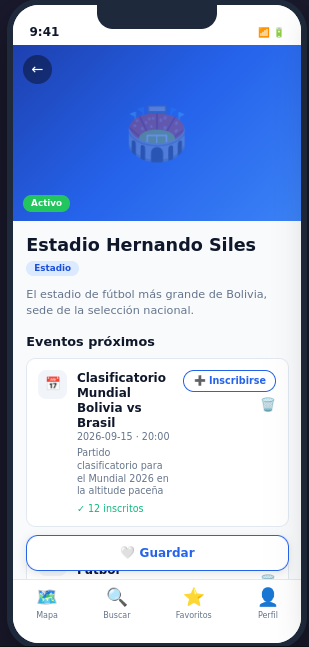
\includegraphics[width=0.45\linewidth]{evidencia-boton-inscripcion.png}%
  }{Elaboraci\'on propia (captura de la aplicaci\'on m\'ovil).}
\end{figure}

Se observa el bot\'on con estilo de borde azul y el texto
``Inscribirse'', indicando que el usuario a\'un no est\'a
inscrito en el evento.

\subsection{Evidencia 6: Inscripci\'on exitosa}

Despu\'es de tocar ``Inscribirse'', el bot\'on cambia su estado
visual: fondo azul, texto blanco y icono de checkmark, indicando
que la inscripci\'on fue exitosa.

\begin{figure}[H]
\centering
  \figuraAPA{fig:evidencia-inscrito}{Evidencia: Estado ``Inscrito'' despu\'es de la inscripci\'on exitosa}{%
    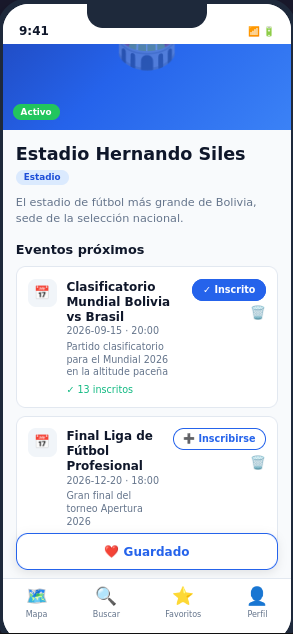
\includegraphics[width=0.45\linewidth]{evidencia-inscrito.png}%
  }{Elaboraci\'on propia (captura de la aplicaci\'on m\'ovil).}
\end{figure}

El conteo de insritos se actualiza autom\'aticamente despu\'es
de la inscripci\'on (ej: ``5 inscritos'' $\to$ ``6 inscritos'').

\subsection{Evidencia 7: Conteo de inscritos actualizado}

Despu\'es de una inscripci\'on, el conteo mostrado debajo del
evento se actualiza en tiempo real gracias a la invalidaci\'on
de cach\'e de React Query.

\begin{figure}[H]
\centering
  \figuraAPA{fig:evidencia-conteo}{Evidencia: Conteo de inscritos actualizado despu\'es de la inscripci\'on}{%
    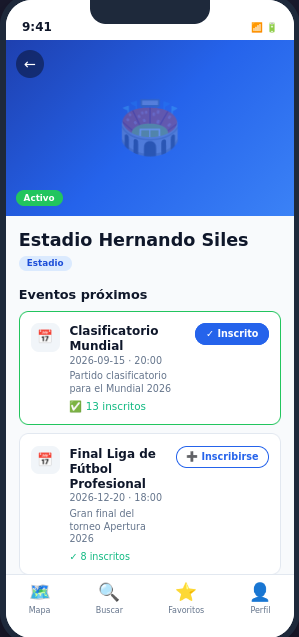
\includegraphics[width=0.45\linewidth]{evidencia-conteo.png}%
  }{Elaboraci\'on propia (captura de la aplicaci\'on m\'ovil).}
\end{figure}

\subsection{Evidencia 8: Confirmaci\'on de cancelaci\'on}

Al tocar el bot\'on ``Inscrito'' para cancelar, se muestra un
di\'alogo de confirmaci\'on para evitar cancelaciones accidentales.

\begin{figure}[H]
\centering
  \figuraAPA{fig:evidencia-cancelar}{Evidencia: Di\'alogo de confirmaci\'on al cancelar inscripci\'on}{%
    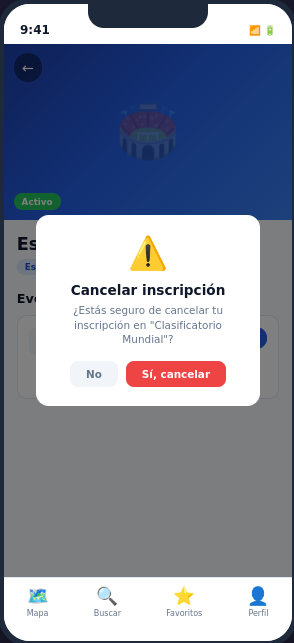
\includegraphics[width=0.40\linewidth]{evidencia-cancelar.png}%
  }{Elaboraci\'on propia (captura de la aplicaci\'on m\'ovil).}
\end{figure}

El usuario tiene dos opciones: ``No'' (mantiene la inscripci\'on)
o ``S\'i, cancelar'' (elimina la inscripci\'on).

\subsection{Evidencia 9: Secci\'on ``Mis inscripciones'' en el perfil}

En la pantalla de perfil del usuario, se muestra la secci\'on
``Mis inscripciones a eventos'' con todas las inscripciones activas.

\begin{figure}[H]
\centering
  \figuraAPA{fig:evidencia-perfil-inscripciones}{Evidencia: Secci\'on ``Mis inscripciones'' en la pantalla de perfil}{%
    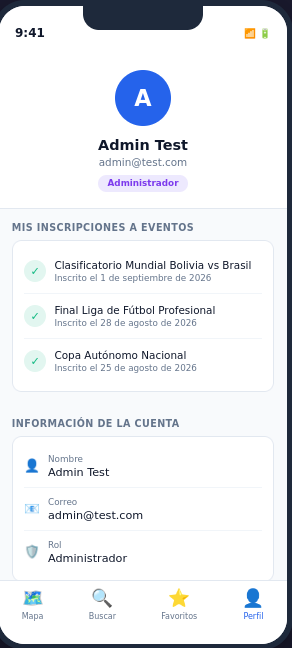
\includegraphics[width=0.45\linewidth]{evidencia-perfil-inscripciones.png}%
  }{Elaboraci\'on propia (captura de la aplicaci\'on m\'ovil).}
\end{figure}

Cada inscripci\'on muestra el icono de confirmaci\'on verde y la
fecha en que se realiz\'o la inscripci\'on.

\subsection{Evidencia 10: Estado vac\'io (sin inscripciones)}

Un usuario que no tiene inscripciones ve un estado vac\'io con
un icono descriptivo y un mensaje informativo.

\begin{figure}[H]
\centering
  \figuraAPA{fig:evidencia-vacio}{Evidencia: Estado vac\'io cuando el usuario no tiene inscripciones}{%
    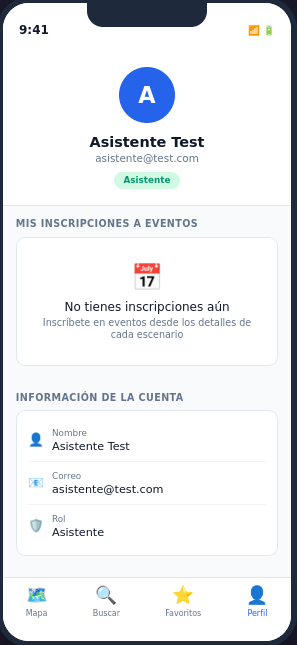
\includegraphics[width=0.45\linewidth]{evidencia-vacio.png}%
  }{Elaboraci\'on propia (captura de la aplicaci\'on m\'ovil).}
\end{figure}

El mensaje ``No tienes inscripciones aun'' orienta al usuario
sobre c\'omo inscribirse desde los detalles de cada escenario.

\subsection{Evidencia 11: Alerta de usuario no autenticado}

Si un usuario no est\'a logueado e intenta inscribirse, se muestra
una alerta indicando que debe iniciar sesi\'on.

\begin{figure}[H]
\centering
  \figuraAPA{fig:evidencia-no-auth}{Evidencia: Alerta para usuario no autenticado}{%
    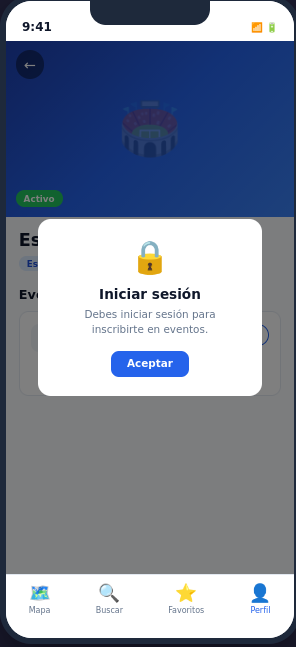
\includegraphics[width=0.40\linewidth]{evidencia-no-auth.png}%
  }{Elaboraci\'on propia (captura de la aplicaci\'on m\'ovil).}
\end{figure}

\subsection{Evidencia 12: Typecheck sin errores}

Se ejecut\'o \texttt{tsc --noEmit} y el proyecto compila
correctamente sin errores de tipo TypeScript.

\begin{figure}[H]
\centering
  \figuraAPA{fig:evidencia-typecheck}{Evidencia: Typecheck exitoso sin errores de TypeScript}{%
    \colorbox{termbg}{%
      \begin{minipage}{0.72\linewidth}
        \color{termfg}\ttfamily\footnotesize
        \textcolor{termcmd}{\$ }\texttt{tsc --noEmit}\\
        \textcolor{termok}{\checkmark}\textcolor{termfg}{ No errors found.}\\[2pt]
        \textcolor{termcmd}{\$ }\texttt{echo \$?}\\
        \textcolor{termout}{0}
      \end{minipage}%
    }%
  }{Elaboraci\'on propia (wireframe de terminal).}
\end{figure}

\subsection{Evidencia 13: Estructura de archivos del m\'odulo}

Los archivos creados/modificados para el m\'odulo se organizan
de la siguiente manera:

\begin{figure}[H]
\centering
  \figuraAPA{fig:evidencia-estructura}{Evidencia: Estructura de archivos del m\'odulo de inscripci\'on}{%
    \begin{tabular}{@{}l@{}}
      \texttt{supabase/migrations/}\\
      \quad \textcolor{termok}{011\_event\_registrations.sql}~\emph{(nuevo)}\\
      \texttt{src/hooks/}\\
      \quad \textcolor{termok}{useEventRegistration.ts}~\emph{(nuevo)}\\
      \texttt{src/types/}\\
      \quad database.ts~\emph{(modificado)}\\
      \quad index.ts~\emph{(modificado)}\\
      \texttt{src/app/}\\
      \quad scenario/[id].tsx~\emph{(modificado)}\\
      \quad (tabs)/profile.tsx~\emph{(modificado)}\\
    \end{tabular}%
  }{Elaboraci\'on propia (wireframe del explorador de archivos).}
\end{figure}

\subsection{Resumen de archivos creados/modificados}

\begin{table}[H]
\centering
\begin{tabular}{@{}lp{4cm}p{3cm}@{}}
\toprule
\textbf{Archivo} & \textbf{Descripci\'on} & \textbf{Estado} \\
\midrule
011\_event\_registrations.sql & Migraci\'on con tabla y RLS & Nuevo \\
useEventRegistration.ts & Hooks de React Query & Nuevo \\
database.ts & Tipos de Supabase & Modificado \\
index.ts & Tipos TypeScript & Modificado \\
{[}id{]}.tsx & Detalle del escenario & Modificado \\
profile.tsx & Pantalla de perfil & Modificado \\
\bottomrule
\end{tabular}
\caption{Archivos del m\'odulo de inscripci\'on}
\end{table}

\subsection{Evidencia 14: Git diff de los cambios}

El repositorio muestra los cambios realizados en la rama
\texttt{feature/event-registration}:

\begin{figure}[H]
\centering
  \figuraAPA{fig:evidencia-git}{Evidencia: Estado de Git con los archivos modificados}{%
    \colorbox{termbg}{%
      \begin{minipage}{0.72\linewidth}
        \color{termfg}\ttfamily\footnotesize
        \textcolor{termcmd}{On branch}\textcolor{termfg}{ feature/event-registration}\\[2pt]
        \textcolor{termok}{Changes not staged for commit:}\\
        \quad \texttt{modified: src/app/scenario/[id].tsx}\\
        \quad \texttt{modified: src/app/(tabs)/profile.tsx}\\[2pt]
        \textcolor{termok}{Untracked files:}\\
        \quad \texttt{src/hooks/useEventRegistration.ts}\\
        \quad \texttt{supabase/migrations/011\_...sql}
      \end{minipage}%
    }%
  }{Elaboraci\'on propia (wireframe de terminal con \texttt{git status}).}
\end{figure}

% ============================================================================
%  CONCLUSIONES
% ============================================================================
\newpage
\encabezadoCapitulo{CONCLUSIONES}{}
\addcontentsline{toc}{part}{CONCLUSIONES}

\section{Conclusiones}

El desarrollo del m\'odulo de inscripci\'on a eventos deportivos en
la aplicaci\'on \nombreApp{} demuestra la integraci\'on exitosa de
m\'ultiples conocimientos trabajados durante la materia de
Aplicaciones M\'oviles I:

\begin{enumerate}
  \item \textbf{An\'alisis y dise\~no:} Se identific\'o la necesidad
    de un mecanismo de inscripci\'on a eventos, se defini\'o la
    funcionalidad, y se dise\~naron las interfaces manteniendo la
    consistencia visual del proyecto.

  \item \textbf{Implementaci\'on de interfaz:} Se crearon nuevos
    componentes (\texttt{EventRegistrationButton},
    \texttt{MyRegistrationsSection}) que se integran
    arm\'onicamente con la aplicaci\'on existente.

  \item \textbf{Navegaci\'on:} El m\'odulo se accede desde la
    pantalla de detalle del escenario (secci\'on de eventos) y
    desde la pantalla de perfil (secci\'on ``Mis inscripciones'').

  \item \textbf{L\'ogica de negocio:} Las operaciones de
    inscripci\'on, cancelaci\'on y consulta se implementaron
    mediante hooks personalizados de React Query.

  \item \textbf{Validaciones:} Se implementaron validaciones de
    autenticaci\'on, duplicados, integridad referencial y
    confirmaci\'on de acci\'on.

  \item \textbf{Manejo de estado:} React Query gestiona
    eficientemente el estado del servidor, la cach\'e y la
    invalidaci\'on selectiva.

  \item \textbf{Persistencia:} Toda la informaci\'on se almacena
    en Supabase (PostgreSQL) con pol\'iticas RLS granulares.

  \item \textbf{CRUD:} Se implementaron operaciones CREATE, READ
    y DELETE sobre la tabla \texttt{event\_registrations}.

  \item \textbf{Manejo de errores:} Se contemplaron errores de
    red, datos inv\'alidos, duplicados y usuarios no
    autenticados.

  \item \textbf{Integraci\'on:} El m\'odulo forma parte
    integral de la aplicaci\'on y no funciona como un proyecto
    independiente.
\end{enumerate}

El m\'odulo cumple con todos los requisitos m\'inimos establecidos
en la gu\'ia del examen integrador (PDF~7) y demuestra la
capacidad de resolver un desaf\'io real de desarrollo de software
m\'ovil utilizando las tecnolog\'ias trabajadas durante la materia.

% ============================================================================
%  REFERENCIAS
% ============================================================================
\newpage
\encabezadoCapitulo{REFERENCIAS}{}
\addcontentsline{toc}{part}{REFERENCIAS}

\bibliographystyle{apacite}
\nocite{*}

\begin{thebibliography}{99}

\bibitem[\protect\citeauthoryear{Pressman}{Pressman}{2010}]{pressman2010}
Pressman, R.~S. (2010). \textit{Ingenier{\'\i}a del software: un enfoque pr\'actico (7.{\textordfeminine} ed.)}. McGraw-Hill.

\bibitem[\protect\citeauthoryear{Sommerville}{Sommerville}{2011}]{sommerville2011}
Sommerville, I. (2011). \textit{Ingenier\'ia de software (9.{\textordfeminine} ed.)}. Pearson Educaci\'on.

\bibitem[\protect\citeauthoryear{Hern\'andez Sampieri et al.}{Hern\'andez Sampieri, Fern\'andez Collado, and Baptista Lucio}{2014}]{hernandez2014}
Hern\'andez Sampieri, R., Fern\'andez Collado, C., y Baptista Lucio, M.~d.~P. (2014). \textit{Metodolog\'ia de la investigaci\'on (6.{\textordfeminine} ed.)}. McGraw-Hill.

\bibitem[\protect\citeauthoryear{Arias}{Arias}{2012}]{arias2012}
Arias, F.~G. (2012). \textit{El proyecto de investigaci\'on: introducci\'on a la metodolog\'ia cient\'ifica (6.{\textordfeminine} ed.)}. Editorial Episteme.

\bibitem[\protect\citeauthoryear{Kendall and Kendall}{Kendall and Kendall}{2011}]{kendall2011}
Kendall, K.~E. y Kendall, J.~E. (2011). \textit{An\'alisis y dise\~no de sistemas (8.{\textordfeminine} ed.)}. Pearson Educaci\'on.

\bibitem[\protect\citeauthoryear{Nielsen}{Nielsen}{1994}]{nielsen1994}
Nielsen, J. (1994). \textit{Usability engineering}. Morgan Kaufmann.

\bibitem[\protect\citeauthoryear{Longley et al.}{Longley, Goodchild, Maguire, and Rhind}{2015}]{longley2015}
Longley, P.~A., Goodchild, M.~F., Maguire, D.~J., y Rhind, D.~W. (2015). \textit{Geographic information science and systems (4.{\textordfeminine} ed.)}. Wiley.

\bibitem[\protect\citeauthoryear{Larman}{Larman}{2004}]{larman2004}
Larman, C. (2004). \textit{Applying UML and patterns: an introduction to object-oriented analysis and design and iterative development (3.{\textordfeminine} ed.)}. Prentice Hall.

\bibitem[\protect\citeauthoryear{ISO}{ISO}{2011}]{iso25010}
International Organization for Standardization. (2011). \textit{ISO/IEC 25010:2011, Systems and software engineering --- Systems and software quality requirements and evaluation (SQuaRE) --- System and software quality models}. Ginebra, Suiza.

\bibitem[\protect\citeauthoryear{Meta Platforms}{Meta Platforms}{2026}]{reactnative}
Meta Platforms. (2026). \textit{React Native: documentaci\'on oficial}. Recuperado de \url{https://reactnative.dev/}

\bibitem[\protect\citeauthoryear{Expo}{Expo}{2026}]{expo}
Expo. (2026). \textit{Expo: documentaci\'on oficial}. Recuperado de \url{https://docs.expo.dev/}

\bibitem[\protect\citeauthoryear{OpenJS Foundation}{OpenJS Foundation}{2026}]{nodejs}
OpenJS Foundation. (2026). \textit{Node.js: documentaci\'on oficial}. Recuperado de \url{https://nodejs.org/es/docs/}

\bibitem[\protect\citeauthoryear{PostgreSQL Global Development Group}{PostgreSQL Global Development Group}{2026}]{postgresql}
PostgreSQL Global Development Group. (2026). \textit{PostgreSQL: documentaci\'on oficial}. Recuperado de \url{https://www.postgresql.org/docs/}

\bibitem[\protect\citeauthoryear{Supabase}{Supabase}{2026}]{supabase}
Supabase. (2026). \textit{Supabase: documentaci\'on oficial}. Recuperado de \url{https://supabase.com/docs}

\bibitem[\protect\citeauthoryear{Leaflet}{Leaflet}{2026}]{leaflet}
Leaflet. (2026). \textit{Leaflet: an open-source JavaScript library for mobile-friendly interactive maps}. Recuperado de \url{https://leafletjs.com/}

\bibitem[\protect\citeauthoryear{Estado Plurinacional de Bolivia}{Estado Plurinacional de Bolivia}{2009}]{cpe2009}
Estado Plurinacional de Bolivia. (2009). \textit{Constituci\'on Pol\'itica del Estado Plurinacional de Bolivia}. La Paz, Bolivia.

\bibitem[\protect\citeauthoryear{Estado Plurinacional de Bolivia}{Estado Plurinacional de Bolivia}{2012}]{ley277}
Estado Plurinacional de Bolivia. (2012). \textit{Ley N.{\textordmasculine} 277 de 2012, Ley del Deporte}. La Paz, Bolivia.

\bibitem[\protect\citeauthoryear{Estado Plurinacional de Bolivia}{Estado Plurinacional de Bolivia}{2011}]{ley164}
Estado Plurinacional de Bolivia. (2011). \textit{Ley N.{\textordmasculine} 164 de 2011, Ley General de Telecomunicaciones, Tecnolog\'ias de Informaci\'on y Comunicaci\'on}. La Paz, Bolivia.

\bibitem[\protect\citeauthoryear{Google}{Google}{2026}]{androidstudio}
Google. (2026). \textit{Android Studio: the official IDE for Android}. Recuperado de \url{https://developer.android.com/studio}

\bibitem[\protect\citeauthoryear{Git}{Git}{2026}]{gitdocs}
Git. (2026). \textit{Git: documentaci\'on oficial}. Recuperado de \url{https://git-scm.com/doc}

\bibitem[\protect\citeauthoryear{GitHub}{GitHub}{2026}]{githubdocs}
GitHub. (2026). \textit{GitHub Docs}. Recuperado de \url{https://docs.github.com/}

\bibitem[\protect\citeauthoryear{Schwaber and Sutherland}{Schwaber and Sutherland}{2020}]{schwaber2020}
Schwaber, K. y Sutherland, J. (2020). \textit{La Gu{\'\i}a de Scrum: la gu{\'\i}a definitiva de Scrum: las reglas del juego}. Scrum.org. Recuperado de \url{https://scrumguides.org/}

\bibitem[\protect\citeauthoryear{Beck et al.}{Beck, Beedle, van Bennekum, Cockburn, Cunningham, et al.}{2001}]{beck2001}
Beck, K., Beedle, M., van Bennekum, A., Cockburn, A., Cunningham, W., et~al. (2001). \textit{Manifiesto por el Desarrollo {\'A}gil de Software}. Recuperado de \url{https://agilemanifesto.org/iso/es/manifesto.html}

\bibitem[\protect\citeauthoryear{Cohn}{Cohn}{2004}]{cohn2004}
Cohn, M. (2004). \textit{User Stories Applied: For Agile Software Development}. Addison-Wesley.

\bibitem[\protect\citeauthoryear{React Native Community}{React Native Community}{2026}]{asyncstorage}
React Native Community. (2026). \textit{AsyncStorage: documentaci\'on oficial}. Recuperado de \url{https://react-native-async-storage.github.io/async-storage/}

\bibitem[\protect\citeauthoryear{TanStack}{TanStack}{2026}]{reactquery}
TanStack. (2026). \textit{TanStack Query: documentaci\'on oficial}. Recuperado de \url{https://tanstack.com/query/latest}

\bibitem[\protect\citeauthoryear{Supabase}{Supabase}{2026a}]{supabaseauth}
Supabase. (2026). \textit{Supabase Auth: autenticaci\'on y autorizaci\'on}. Recuperado de \url{https://supabase.com/docs/guides/auth}

\bibitem[\protect\citeauthoryear{Supabase}{Supabase}{2026b}]{supabaserls}
Supabase. (2026). \textit{Row Level Security en Supabase}. Recuperado de \url{https://supabase.com/docs/guides/database/tables#row-level-security}

\bibitem[\protect\citeauthoryear{Colinhacks}{Colinhacks}{2026}]{zod}
Colinhacks. (2026). \textit{Zod: documentaci\'on oficial}. Recuperado de \url{https://zod.dev/}

\end{thebibliography}

\end{document}
